%%
% Please see http://mirror.ox.ac.uk/sites/ctan.org/macros/latex/contrib/beamer/doc/beameruserguide.pdf
%%
%\documentclass[ngerman]{beamer}
\documentclass[english,aspectratio=169]{beamer}

%\usepackage{pgfpages}
%\setbeameroption{second mode text on second screen=right}

\usepackage{mathptmx}
\usepackage[T1]{fontenc}
\usepackage[utf8]{inputenc}
\setlength{\parskip}{\smallskipamount}
\setlength{\parindent}{0pt}
\usepackage{mathtools}
\usepackage{amstext}
%\usepackage{amssymb}
\usepackage{cancel}
\usepackage{stmaryrd}
\usepackage{graphicx}
\usepackage{babel}
\usepackage{isotope}
\usepackage{adjustbox}
%\usepackage{spot}
\usepackage{hyperref}

\usepackage{todo}
%\usepackage{pdfcomment}

%\usepackage{trace}

\usepackage{listings}

% Line-number = input-line-number + gaps between different line-ranges
% http://tex.stackexchange.com/a/297349/28879
\def\lst@MSkipToFirst{%
    \global\advance\lst@lineno\@ne
    \ifnum \lst@lineno=\lst@firstline
        \def\lst@next{\lst@LeaveMode \global\lst@newlines\z@
        \lst@OnceAtEOL \global\let\lst@OnceAtEOL\@empty
        \ifnum \c@lstnumber>0
            \vspace{2 mm}
        \fi
        \lst@InitLstNumber % Added to work with modified \lsthk@PreInit.
        \lsthk@InitVarsBOL
        \c@lstnumber=\numexpr-1+\lst@lineno % this enforces the displayed line numbers to always be the input line numbers
        \lst@BOLGobble}%
        \expandafter\lst@next
    \fi}
% lstinline should have same size as surrounding text:
% http://tex.stackexchange.com/a/161551/28879
\lstdefinestyle{mystyle}{
  basicstyle=%
%    \ttfamily%
%    \lst@ifdisplaystyle\scriptsize\fi
    ,
%  keywordstyle=\color{black}\bfseries,
  breaklines=true,
  showstringspaces=false
}

\lstset{%
	style=mystyle,
    mathescape=false
}

\lstdefinelanguage{posh}%
  {morekeywords={-replace},%
   sensitive=false,%
   %alsoother={$},%
   morecomment=[l]\#,%
   morecomment=[n]{\#=}{=\#},%
   morestring=[s]{"}{"},%
   morestring=[m]{'}{'},%
}[keywords,comments,strings]%

%\makeatletter
%%%%%%%%%%%%%%%%%%%%%%%%%%%%%% Textclass specific LaTeX commands.
% this default might be overridden by plain title style
%\newcommand\makebeamertitle{\frame{\maketitle}}%
% (ERT) argument for the TOC
%\AtBeginDocument{%
%  \let\origtableofcontents=\tableofcontents
%  \def\tableofcontents{\@ifnextchar[{\origtableofcontents}{\gobbletableofcontents}}
%  \def\gobbletableofcontents#1{\origtableofcontents}
%}

%%%%%%%%%%%%%%%%%%%%%%%%%%%%%% User specified LaTeX commands.

%\usetheme{Copenhagen}
%\useoutertheme{shadow}
\usetheme[hideothersubsections]{Hannover}
%\usetheme{Hannover}

%\usepackage{fontspec}

%\setsansfont{Arial}

%\setmainfont{Arial}
%\setsansfont{Fira Sans}
%\setmonofont{Fira Mono}


%\setmainfont{Museo 500}[BoldFont=Museo 700]
%\setsansfont{Museo Sans 500}
%\setmonofont{Museo Sans 500}

\setbeamercovered{transparent}

% Folienzahlen
\setbeamertemplate{footline}
{%
\begin{beamercolorbox}[wd=0.5\textwidth,ht=3ex,dp=1.5ex,leftskip=.5em,rightskip=.5em]{author in head/foot}%
\usebeamerfont{author in head/foot}%
%\insertframenumber{} / \inserttotalframenumber\hfill\insertshortauthor%
\insertframenumber{} / \insertmainframenumber{}\hfill\insertshortauthor%
\end{beamercolorbox}%
\vspace*{-4.5ex}\hspace*{0.5\textwidth}%
\begin{beamercolorbox}[wd=0.5\textwidth,ht=3ex,dp=1.5ex,left,leftskip=.5em]{title in head/foot}%
\usebeamerfont{title in head/foot}%
%\insertshorttitle%
\url{https://github.com/TheConstructor/Presentations}%
\end{beamercolorbox}%
}

% Folienzahlen 2
%\usepackage{textpos} % package for the positioning
%\addtobeamertemplate{frametitle}{}{%
%\begin{textblock*}{100mm}(\textwidth,-1\baselineskip)
%\insertframenumber{}
%\end{textblock*}}

% Keine Navigationssymbole
\setbeamertemplate{navigation symbols}{}

\setbeamertemplate{background canvas}[vertical shading][]

%\makeatother

\global\long\def\iso#1#2#3{\isotope[#1][#2]{#3}}%
\global\long\def\e{\text{e}}%
\global\long\def\Z{\mathbb{Z}}%
\global\long\def\B{\mathcal{B}}%
\global\long\def\rclass#1{\left\llbracket #1\right\rrbracket }%

\title[Introduction To Regular Expressions]{Taming The Dragon:\\
An Introduction To Regular Expressions}
\author[M. Vill]{Matthias~Vill}
\institute[NSD 2020]{New Stars of Data 2020}
\date{14-Aug-2020}
% \titlegraphic{\includegraphics[height=0.5cm]{graphics/wwu-logo-neu}\hphantom{mm}\includegraphics[height=0.5cm]{graphics/cs_logo_nl_blue}\hphantom{mm}\includegraphics[height=0.5cm]{graphics/comsys_logo}}

%\pgfdeclareimage[height=0.5cm]{institution-logo}{graphics/comsys_logo}
%\logo{\pgfuseimage{institution-logo}}

%\AtBeginSubsection[]{%
%  \frame<beamer>{ 
%    \frametitle{Gliederung}   
%    \tableofcontents[currentsection,currentsubsection] 
%  }
%}

%\AtBeginSection[]{%
%%  \frame<beamer>{\sectionpage}
%  \frame<beamer>{ 
%    \frametitle{Agenda of \insertsection}
%    %\tableofcontents[currentsection,hideothersubsections] 
%    \tableofcontents[sectionstyle=show/hide,subsectionstyle=show/show/hide]
%  }
%}


%\beamerdefaultoverlayspecification{<+->}

\begin{document}

\frame{\maketitle}

{
   \usebackgroundtemplate{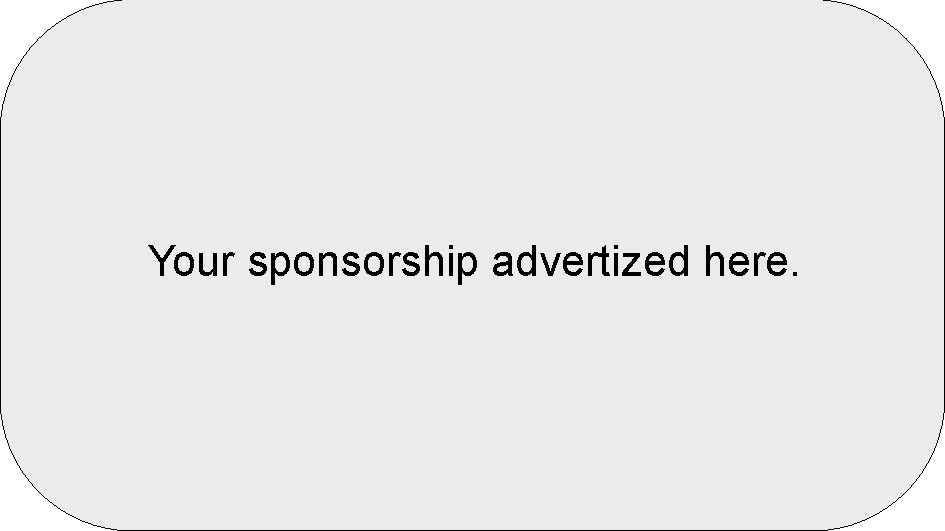
\includegraphics[height=\paperheight]{graphics/Sponsors}}
   %\frame[plain,noframenumbering]{}
   \frame[plain]{}
}

\subsection*{Agenda}
\begin{frame}{Agenda}
    \tableofcontents[hideallsubsections]
\end{frame}

\section{Overview}

\subsection{Introduction}
\begin{frame}{About me}
\begin{columns}
    \column{.75\textwidth}
        \begin{itemize}
            \item Aged 33
            \item Diplom-Informatiker ($\simeq$ Master in Computer Science)
            \item First contact with coding in the 90s (VB 3.1)
            \item First contact with Regular Expressions and (My)SQL through PHP around 2000
            \item Currently employed as Software Developer with focus on T-SQL, but also using C\# and PowerShell
            \item Experience in Java, Bash-, BAT-scripting, Ruby, \textellipsis
        \end{itemize}
        \begin{center}
            \hyperlink{https://www.youracclaim.com/badges/bd81bbb0-8416-40b7-bede-77e7f2b0d5cf}{\adjustimage{max width={1.0\columnwidth},max height={2cm},keepaspectratio}{graphics/MCSA} }
        \end{center}
    \column{.25\textwidth}
        \begin{center}
            \adjustimage{max width={1.0\columnwidth},max height={6cm},keepaspectratio}{graphics/A_054265} 
        \end{center}
    \end{columns}
\end{frame}

\begin{frame}{Regular Expressions}

\begin{itemize}
% \item Two articles in the PHP Magazin (2002.1/2002.2) by Alexander Aulbach started my journey with Regular Expressions
% \item There are multiple flavours of RegExp
\item IEEE POSIX defines 3 flavours: \cite{wiki}\\
    \begin{itemize}
    \item BRE (Basic Regular Expressions)
    \item ERE (Extended Regular Expressions)
    \item  SRE (Simple Regular Expressions; deprecated)
    \end{itemize}
\item Closest to being the goto might be PCRE (= Perl Compatible Regular Expressions; similar to ERE) \cite{wikiPCRE, pcre2syntax}
\item Like with SQL many things can easily be applied to most implementations
\item \textbf{Note:} I will use a \textdagger{} to denote 'unsafe' stuff
\end{itemize}
\end{frame}

\begin{frame}{Idea \& Applications}

\begin{columns}
    \column{.60\textwidth}
        \begin{itemize}
        \item Mathematical roots
        \item It is common to search in strings
        \begin{itemize}
        \item needing more than a literal-match
        \item not wanting a dedicated parser
        \end{itemize}
        \item Flexibility comes at a price
        \item Not for everything, but often handy
        \end{itemize}
    \column{.40\textwidth}
        \begin{center}
            \adjustimage{max width={1.0\columnwidth},max height={8cm},keepaspectratio}{graphics/Multitool}
        \end{center}
    \end{columns}
\end{frame}

\section{Building blocks}
\begin{frame}{Building Blocks}
\begin{columns}
    \column{.75\textwidth}
        Regular Expressions are made up of
        \begin{itemize}
            \item \textbf{Literals}, matching themself
            \item \textbf{Classes}, matching one character out of a list
            \item \textbf{Quantifiers}, saying how often to match
            \item \textbf{Groups}, to treat sections separately
            \item \textbf{Anchors} and \textbf{Asserts}, aligning the match to the 'outside'
            \item and a few other things
        \end{itemize}
    \column{.25\textwidth}
        \begin{center}
            \adjustimage{max width={1.0\columnwidth},max height={6cm},keepaspectratio}{graphics/BuildingBlocks}%
        \end{center}
\end{columns}
\end{frame}

\subsection{Literals}
\begin{frame}{Literals}
\begin{columns}
    \column{.75\textwidth}
        Regular Expressions have escaping similar to C
        \begin{itemize}
            \item most characters are literals (exceptions covered on the next slides)
            \item \texttt{\textbackslash} used to escape special characters and introduce special stuff
            \item \texttt{\textbackslash{}\textbackslash}, \texttt{\textbackslash{}r}, \texttt{\textbackslash{}n}, \texttt{\textbackslash{}t} like C/JSON/...: backslash, carriage return, line feed, tab
        \end{itemize}
    \column{.25\textwidth}
        \begin{center}
            \adjustimage{max width={1.0\columnwidth},max height={6cm},keepaspectratio}{graphics/BuildingBlocksLiterals}%
        \end{center}
\end{columns}
\end{frame}

\subsection{Classes}
\begin{frame}{Classes}
\begin{columns}
    \column{.75\textwidth}
        You probably know classes from T-SQL's \texttt{LIKE}, but RegExp support a few predefined classes
        \begin{itemize}
            \item \texttt{[acd]} matches \texttt{a}, \texttt{c} or \texttt{d}
            \item \texttt{[\string^acd]} matches a character except \texttt{a}, \texttt{c} or \texttt{d}
            \item \texttt{[a-d]} matches \texttt{a}, \texttt{b}, \texttt{c} or \texttt{d}
            \item \texttt{.} may\textdagger{} not match line-breaks, but everything else
            \item \texttt{\string\d} matches digits\textdagger{} (Unicode?!)
            \item \texttt{\string\w} matches 'word'-letters\textdagger{} (\texttt{[a-zA-Z0-9\_]})
            \item \texttt{\string\s} matches white-space
            \item \texttt{\string\S} matches non-white-space
            \item<2-> \texttt{[\string\da-fA-F]} matches hex-digits\textdagger{} (or \texttt{[\string0-9a-fA-F]})
            \item<2-> refer to your implementation's documentation for more
        \end{itemize}
    \column{.25\textwidth}
        \begin{center}
            \adjustimage{max width={1.0\columnwidth},max height={6cm},keepaspectratio}{graphics/BuildingBlocksClasses}%
        \end{center}
\end{columns}
\end{frame}

\subsection{Quantifiers}
\begin{frame}{Quantifiers}
\begin{columns}
    \column{.75\textwidth}
        Things tend to repeat themselves. A lot.
        \begin{itemize}
            \item \texttt{a?}: there will be one \textbf{a} or no \textbf{a}
            \item \texttt{a+}: there will be one \textbf{a} or more
            \item \texttt{a*}: there will be any number of \textbf{a}s or none
            \item \texttt{a\string{0,1\string}}: there will be between 0 and 1 \textbf{a}
            \item \texttt{a\string{1,\string}}: there will be one \textbf{a} or more
            \item \texttt{a\string{3\string}}: there will be three \textbf{a}s
            \item<2-> \textit{special}: \texttt{a??}, \texttt{a+?}, \texttt{a*?} and \texttt{\string{\string}?} prefer fewer \textbf{a}s ('non-greedy'/reluctant)
            \item<2-> \textit{special}: \texttt{a?+}, \texttt{a++}, \texttt{a*+} and \texttt{\string{\string}+} don't back-track (possessive)
        \end{itemize}
    \column{.25\textwidth}
        \begin{center}
            \adjustimage{max width={1.0\columnwidth},max height={6cm},keepaspectratio}{graphics/BuildingBlocksQuantors}%
        \end{center}
\end{columns}
\end{frame}

\subsection{Groups}
\begin{frame}{Groups}
\begin{columns}
    \column{.75\textwidth}
        By themselves they don't do much, but you can use them to
        \begin{itemize}
            \item later refer to them: \\
            \begin{itemize}
                \item \texttt{(['"])a\string\1}; in replacement \texttt{\$1}
                \item \texttt{(?<q>['"])a\string\k<q>} \textdagger{}; in replacement \texttt{\$\{q\}} \textdagger{} \cite{CIUnamedGroups}
            \end{itemize}
            \item have alternatives: \texttt{(ac|dc)}
            \item do styling: \texttt{(?:looks good\string\?)}
            \item change options: \texttt{(?i:sql)} or \texttt{(?-i)sql}
            \item repeat sections: \texttt{(?:[ad]c)*}
        \end{itemize}
        \uncover<2->{Noticed the \texttt{?} at the beginning of some group-types?}
    \column{.25\textwidth}
        \begin{center}
            \adjustimage{max width={1.0\columnwidth},max height={6cm},keepaspectratio}{graphics/BuildingBlocksGroups}%
        \end{center}
\end{columns}
\end{frame}

\subsection{Anchors and Asserts}
\begin{frame}{Anchors and Asserts}
\begin{columns}
    \column{.75\textwidth}
        When something has to be there, but \textellipsis
        \begin{itemize}
            \item \texttt{\string^a}: \textbf{a} should be the first thing (on a line)
            \item \texttt{a\$}: \textbf{a} should be the last thing (on a line)
            \item \texttt{a\string\b}: \textbf{a} should be at the end of a word\textdagger{}
            \item \texttt{/(?=DC)}: \textbf{DC} should come after \textbf{/}
            \item \texttt{/(?!AC)}: \textbf{AC} should not come after \textbf{/}
            \item \texttt{(?<=AC)/}: \textbf{AC} should come before \textbf{/}
            \item \texttt{(?<!DC)/}: \textbf{DC} should not come before \textbf{/}
        \end{itemize}
    \column{.25\textwidth}
        \begin{center}
            \adjustimage{max width={1.0\columnwidth},max height={6cm},keepaspectratio}{graphics/BuildingBlocksAnchors}%
        \end{center}
\end{columns}
\end{frame}

\section{Regular Expressions}

\subsection{Note}
\begin{frame}{Note}
\begin{columns}
    \column{.60\textwidth}
        Let's see some Regular Expressions.
        \begin{itemize}
        \item Focus is on common usage
        \item It is easier to write Regular Expressions, than to read them
        \item Be aware of your context - you might need additional escapes
        \item Regular Expressions are programming: do at least some testing!
        \item Don't give up
        \end{itemize}
    \column{.40\textwidth}
        \begin{center}
            \adjustimage{max width={1.0\columnwidth},max height={6cm},keepaspectratio}{graphics/common}%
        \end{center}
\end{columns}
\end{frame}

\subsection{In your editor}
\begin{frame}{In your editor}

\begin{itemize}
\item If you are using a Microsoft/JetBrains editor/IDE: look for \texttt{.*} near the pattern input \\
        \begin{center}
            \adjustimage{max width={1.0\columnwidth},max height={1cm},keepaspectratio}{graphics/ADSsearch}
            \adjustimage{max width={1.0\columnwidth},max height={1cm},keepaspectratio}{graphics/DGsearch}
        \end{center}
\item Notepad++ has 'Search Mode' at the bottom \\
        \begin{center}
            \adjustimage{max width={1.0\columnwidth},max height={1.5cm},keepaspectratio}{graphics/NPPsearch}%
        \end{center}
\item \textellipsis
\end{itemize}
\end{frame}

\subsection{In your code}
\begin{frame}{In your code}
These are only examples!
\begin{itemize}
\item PowerShell:
    \begin{itemize}
    \item \texttt{'CONTOSO\textbackslash{}Bob' -replace '\textbackslash{}w+\textbackslash{}\textbackslash{}(?<user>\textbackslash{}w+)', 'FABRIKAM\textbackslash{}\textdollar{}\string{user\string}'}
    \item \texttt{Select-String -Path .\textbackslash{}*.sql -Pattern 'FROM\textbackslash{}s+(\textbackslash{}S+)'}
    \end{itemize}
\item C\#:
    \begin{itemize}
    \item \texttt{Regex.Replace("CONTOSO\textbackslash{}\textbackslash{}Bob","\textbackslash{}\textbackslash{}w+\textbackslash{}\textbackslash{}\textbackslash{}\textbackslash{}(?<user>\textbackslash{}\textbackslash{}w+)", "FABRIKAM\textbackslash{}\textbackslash{}\textdollar{}\{user\}");}
    \item \texttt{Directory.EnumerateFiles(".", "*.sql")\\
    .Select(f => (f, c: File.ReadLines(f)))\\
    .SelectMany(t => t.c.Select((l,n) => (t.f, n, m: Regex.Match(l, @"FROM\textbackslash{}s+(\textbackslash{}S+)")))\\
        .Where(mt => mt.m.Success))}
    \end{itemize}
\end{itemize}
\end{frame}

\begin{frame}[fragile]{In your code}
\begin{itemize}
\item MySQL 8:
    \begin{itemize}
    \item \lstinline[language=SQL]!SELECT REGEXP_REPLACE('CONTOSO\\Bob', '\w+\\\\(?<user>\w+)', 'FABRIKAM\\${user}');!
    \item \begin{lstlisting}[language=SQL]
SET @Haystack := 'SELECT * FROM Demo1; SELECT * FROM Demo2;';
SET @Pattern := 'FROM\\s+(\\S+)';
WITH RECURSIVE Matches AS (
    SELECT 1 AS Num,
        REGEXP_INSTR(@Haystack, @Pattern, 1, 1) AS Pos,
        REGEXP_SUBSTR(@Haystack, @Pattern, 1, 1) AS Str
    UNION ALL SELECT M.Num + 1,
        REGEXP_INSTR(@Haystack, @Pattern, 1, M.Num + 1),
        REGEXP_SUBSTR(@Haystack, @Pattern, 1, M.Num + 1)
    FROM Matches M WHERE M.Pos > 0)
SELECT * FROM Matches M
    \end{lstlisting}
    \end{itemize}
\item \textellipsis
\end{itemize}
\end{frame}

\subsection{Input Validation}
\begin{frame}{Input Validation}
\begin{columns}
    \column{.75\textwidth}
        \begin{itemize}
        \item 'Our serial numbers always have 6 hex-digits'\\
            \visible<2->{\texttt{\string^[0-9a-fA-F]\{6\}\$}}
        \item<3-> 'Names are made of two parts with a space in between'\textdagger\\
            \visible<4->{\texttt{\string^(\string\S+) (\string\S+)\$}}
        \item<5-> '\textbf{a} is repeated an "unprime" number of times'\\
            \visible<6->{\texttt{\string^(a\{2,\}?)\textbackslash1++\$}}
        \item<7-> 'It is a valid E-Mail-address'\\
            \begin{visibleenv}<8->
                There is a RegExp implementing \href{https://www.rfc-editor.org/rfc/rfc822.html\#section-6.1}{RFC822} available at \url{https://www.ex-parrot.com/pdw/Mail-RFC822-Address.html}. \href{https://stackoverflow.com/a/20773069/1266906}{A SO-answer} suggests to check for an \texttt{@}, then send an E-Mail to verify
            \end{visibleenv}
        \end{itemize}
    \column{.25\textwidth}
        \begin{center}
            \adjustimage{max width={1.0\columnwidth},max height={6cm},keepaspectratio}{graphics/InputValidation}%
        \end{center}
\end{columns}
\end{frame}

\subsection{Editor Tasks - Demos}
\begin{frame}{Editor Tasks - Demos}
\begin{columns}
    \column{.75\textwidth}
        \begin{itemize}
        \item Fold multiple spaces into one
        \item Find all usages of an object in a script (quoted, default schema, \textellipsis)
        \item Rename procedures: CREATE OR ALTER $\xRightarrow{\text{replaced by}}$ DROP IF EXISTS + CREATE OR ALTER
        \item Rewrite UPDATE to INSERT: UPDATE x SET y = ? $\xRightarrow{\text{replaced by}}$ INSERT x (y) VALUES (?)
        \end{itemize}
    \column{.25\textwidth}
        \begin{center}
            \adjustimage{max width={1.0\columnwidth},max height={7cm},keepaspectratio}{graphics/FlyDragon}%
        \end{center}
\end{columns}
\end{frame}

\section{Summary}

%\subsection*{Summary}
\begin{frame}{Summary}
\begin{columns}
    \column{.60\textwidth}
    \begin{itemize}
        \item Regular Expressions are flexible and powerful
        \item MS SQL lacks native RegExp, but CLR can add it
        \item They are often easier to write than to read
        \item As with many things: use the right tool for the job
    \end{itemize}
    \column{.40\textwidth}
        \begin{center}
            \adjustimage{max width={1.0\columnwidth},max height={8cm},keepaspectratio}{graphics/D-svlGFWsAErN5b}%
\\\cite{comicHowToRegex}
        \end{center}
\end{columns}
\end{frame}

\appendix
% Folienzahlen
\setbeamertemplate{footline}
{%
\begin{beamercolorbox}[wd=0.5\textwidth,ht=3ex,dp=1.5ex,leftskip=.5em,rightskip=.5em]{author in head/foot}%
\usebeamerfont{author in head/foot}%
%\insertframenumber{} / \inserttotalframenumber\hfill\insertshortauthor%
\insertframenumber{} / \insertmainframenumber{} + \insertappendixframenumber{}\hfill\insertshortauthor%
\end{beamercolorbox}%
\vspace*{-4.5ex}\hspace*{0.5\textwidth}%
\begin{beamercolorbox}[wd=0.5\textwidth,ht=3ex,dp=1.5ex,left,leftskip=.5em]{title in head/foot}%
\usebeamerfont{title in head/foot}%
\insertshorttitle%
\end{beamercolorbox}%
}
\beamerdefaultoverlayspecification{}

\section*{Apendix}

\subsection*{Feedback}
\begin{frame}{Feedback}
\begin{center}
{\usebeamerfont*{title} \usebeamercolor[fg]{title} Please provide feedback}
\end{center}
\end{frame}

\subsection*{Sources}
\begin{frame}[allowframebreaks]{Sources}

\bibliographystyle{IEEEtran}
\nocite{*}
\bibliography{bibliography}
\end{frame}

\end{document}

